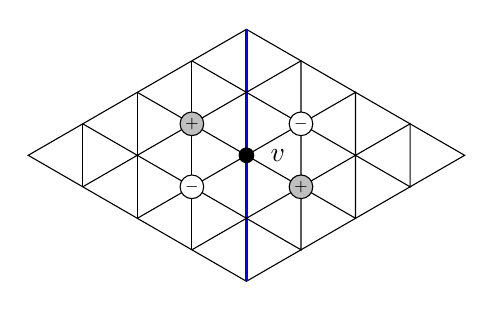
\begin{tikzpicture}[baseline=0cm]
\draw (0,0) -- (30:3.2) -- (90:3.2) -- (150:3.2) -- cycle;
\draw[blue,very thick] (0,0) -- (0,3.2);

\foreach \x in {1,2,3}
\draw (150:{0.8*\x}) edge +(0,{0.8*(4-\x)}) -- ++(30:3.2)
	-- ++(0,{-0.8*\x}) -- ++(150:3.2);

\fill (0,1.6) circle[radius=0.1] ++(0.4,0) node{$v$};
\foreach \t in {30,210}
\draw[fill=white] (0,1.6) ++(\t:0.8)node{\tiny$-$} circle[radius=0.15];
\foreach \t in {150,-30}
\draw[fill=lightgray] (0,1.6) ++(\t:0.8)node{\tiny$+$} circle[radius=0.15];
\end{tikzpicture}